\documentclass[brudnopis]{xmgr}
%\documentclass[xodstep]{xmgr}

%\defaultfontfeatures{Scale=MatchLowercase}
%\setmainfont[Numbers=OldStyle,Ligatures=TeX]{Minion Pro}
%\setsansfont[Numbers=OldStyle,Ligatures=TeX]{Myriad Pro}
% for fontspec version < 2.0
\setmainfont[Numbers=OldStyle,Mapping=tex-text]{Minion Pro}
\setsansfont[Numbers=OldStyle,Mapping=tex-text]{Myriad Pro}
%\setmonofont[Scale=0.75]{Monaco}

% Opcjonalnie identyfikator dokumentu 
% drukowany tylko z włączoną opcją 'brudnopis':
\wersja   {}

\author   {Dorian Sawa}
\nralbumu {186\,445}
\email    {dsawa@sigma.ug.edu.pl}

\title    {System weryfikacji jakości kodu w języku Scala}
\date     {2014}
\miejsce  {Gdańsk}

\opiekun  {dr Wiesław Pawłowski}

% dodatkowe polecenia
%\renewcommand{\filename}[1]{\texttt{#1}}

\begin{document}

\begin{abstract}
Scala to język wspierający paradygmaty programowania obiektowego i funkcyjnego. Rosnąca w ostatnim czasie popularność Scali przyczyniła się do powstania wielu narzędzi pozwalających na testowanie programów napisanych właśnie w tym języku. Niniejsza praca zgłębia temat wspomnianych narzędzi oraz ich wykorzystania jako podstawy systemu pozwalającego na automatyzację kontroli jakości kodu.
\end{abstract}
\keywords{Scala, 
 Play Framework, 
 Scalatest, 
 Scalacheck,
 Scalastyle}

% tytuł i spis treści
\maketitle
%
% wstęp
\introduction Scala jest nowoczesnym językiem programowania działającym na wirtualnej maszynie Javy. Od chwili opublikowania jest ona sukcesywnie rozwijana. Współcześnie wiele firm korzysta z systemów napisanych w Scali. Systemy takie, napisane dla celów wewnętrznych, czy też komercyjnych spełniają swoje zadania z sukcesami. Wśród firm korzystających z technologii Scali znaleźć można między innymi LinkedIn, Twitter czy Intel. Chociaż Scala jest językiem całkowicie zorientowanym obiektowo, to posiada on także wszystkie elementy jakie można oczekiwać od języka funkcyjnego.

Przy wielu zaletach jakie ze sobą niesie możliwość programowania w Scali, udział procentowy tego języka na tle konkurencji wciąż jest stosukowo nieduży. Oczywiście proporcjonalnie do takiego rozkładu wygląda również sytuacja programistów Scali na rynku pracy. Jednym z impulsów do zmiany tego faktu mogłaby być specjalna platforma pozwalająca przyspieszyć proces nauki Scali. Na tym zagadnieniu skupia się niniejsza praca.

Zaprojektowany i opisywany tu system powstał na bazie nowoczesnych technologii oraz najważniejszych narzędzi do testów jednostkowych. Podstawą systemu jest Play Framework. Pozwala on na szybkie napisanie aplikacji internetowej zarówno w Scali jak i w Javie. Społeczność powstała wokół tych dwóch języków doprowadziła do powstania ogromnej liczby bibliotek. Z powodzeniem mogą być one używane w aplikacji utworzonej przy użyciu Play Framework. 

Pośród bibliotek związanych z testowaniem kodu na szczególną uwagę zasługuje Scalatest oraz Scalacheck. Pierwsza z nich to biblioteka do przeprowadzania testów jednostkowych. Umożliwia ona między innymi pisanie testów w wielu różnych stylach. Decyzja o tym jak ostatecznie wyglądać będzie test zależy od preferencji użytkownika. Scalacheck jest zaś instrumentem służącym do testowania funkcji, metod poprzez automatyczne wprowadzanie różnych argumentów. 

Projektując system do weryfikacji kodu Scala zdecydowałem się skorzystać z nierelacyjnej bazy danych z wbudowanym mechanizmem do przechowywania plików - MongoDB. Interfejs użytkownika powstał zaś przy pomocy AngularJS, który w przyjemny dla programisty sposób  potrafi dynamicznie zmieniać zawartość strony HTML warunkując ją od akcji użytkownika mających wpływ na stan modeli aplikacji.

\medskip Na początku swojej pracy postaram się szerzej przedstawić ideę będącą iskrą do stworzenia tego systemu. Pokażę, że dla innych języków programowania już funkcjonują pewne mechanizmy edukacyjne. Kolejnym krokiem będzie prezentacja języka Scala. Opowiem o mechanizmie aktorów, kombinacji języka funkcyjnego i obiektowego oraz innych nowych rzeczach jakie ze sobą niesie. Każde ze wspominanych wcześniej narzędzi zostanie również szerzej przedstawione. Każde z nich wywarło wpływ na ostateczny kształt opisywanej aplikacji. Ustosunkuję się do wyboru tych narzędzi spośród innych. Między innymi dlaczego zdecydowałem się na użycie nierelacyjnego MongoDB. I czemu uznałem, że standardowa funkcjonalność AngularJS to było dla mnie za mało. Ostatecznie przybliżę także sposób działania systemu oraz w jaki sposób użyte zostało jeszcze jedno narzędzie - SBT. Bezpośrednio związane z weryfikacją kodu uczestników systemu. 

\chapter{Idea systemu}

Wykonując odpowiednie zapytanie przy użyciu narzędzia \textit{Google BigQuery} oraz danych z \textit{Github Archive} można w prosty sposób sprawdzić popularność języków programowania na platformie \textit{GitHub}. Ilość repozytoriów dla poszczególnych języków w roku 2013  przedstawia rysunek \ref{RYS.1}. 

\begin{figure}[!tbh]
\centering 
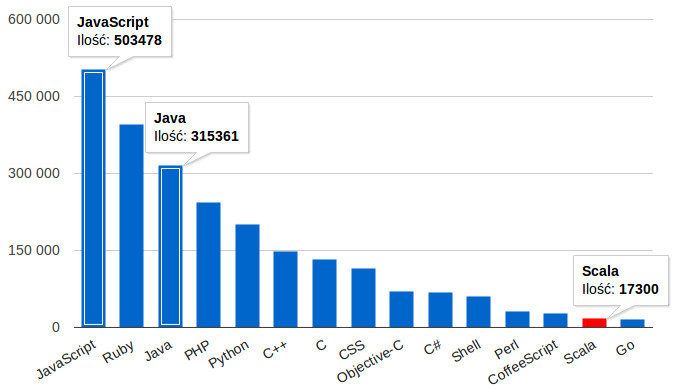
\includegraphics[width=.95\hsize]{fig/top_github_languages_2013}
\caption{Ilość repozytoriów dla poszczegónych języków na platformie GitHub w roku 2013 \label{RYS.1}}
\source{GitHub Archive (www.githubarchive.org)}
\end{figure}

Powyższy wykres przedstawia pierwszych 15 języków, wśród których Scala uplasowała się na miejscu 14. Różnica w liczbie repozytoriów między Scalą, a Javą będącą na trzecim miejscu jest znaczna. Nie ma wątpliwości, że Java swoją wysoką pozycje zawdzięcza wieloletniej obecności na rynku, a także wkładzie jaki do świata technologii informacyjnych wniosła wirtualna maszyna javy. Na popularność JavaScript'u, czy Ruby'ego 
częściowo miało wpływ pojawienie się w ostatniej dekadzie narzędzi takich jak \textit{Ruby on Rails}, \textit{node.js}, \textit{AngularJS} i wielu innych. 

Jednak jak pokazuje przykład Ruby'ego i JavaScriptu, jednym z elementów wpływających na popularność języków jest także swego rodzaju otwartość środowisk zgromadzonych wokół danych języków na możliwość ich nauki. Potwierdzeniem tego może być grupa programistów zgromadzona wokół platformy \textit{CodeSchool}\footnote{www.codeschool.com}. Opracowali oni szereg prostych kursów związanych głownie z JavaScript'em i Ruby'm w trakcie, których uczestnik rozwiązuje proste zadania programistyczne. 

Żadne z obecnych rozwiązań - szczególnie dla Scali - nie posiada jednak możliwości tworzenia własnych zadań dla zamkniętych grup uczestników. Wierzę, że system, który tuż po zaimplementowaniu daje sposobność definiowania własnych kursów dla języka Scala może znacząco zwiększyć jej popularność. Implementacja takiego systemu w szkołach i uczelniach mogłaby przynieść również inne zalety, jak na przykład wzrost zainteresowania programowaniem, czy podniesieniem umiejętności przyszłych programistów przy jednoczesnym mniejszym wysiłku prowadzących zajęcia.

\section{Język Scala}

Stworzenie Scali przypisuje się niemieckiemu profesorowi - Martinowi Oderskiemu. Nazwa ma na celu sugerować, że jest to język skalowalny\footnote{ang: Scalable language}. Scala rośnie wraz z potrzebami jej użytkowników. Cały czas powstają kolejne narzędzia i biblioteki mające uprościć pracę z nią, czy też dodać do niej coś nowego. 

Scala łączy ze sobą paradygmat programowania obiektowego oraz funkcyjnego. Umożliwia wykorzystanie najlepszych cech tych dwóch podejść w projektowaniu nowych systemów. Sprawdzi się zatem doskonale, gdy jest potrzeba zaimplementowania dużego systemu, wymagającego dostosowywania z czasem do nowych potrzeb jak i w przypadku tworzenia mniejszych elementów, gdzie lepiej spisywać będzie się koncepcja programowania funkcyjnego.

\subsection{Scala jako język obiektowy}

Scala jest całkowicie zorientowana obiektowo. Inaczej niż w wielu językach obiektowych, nie posiadamy tutaj wartości, które nie są obiektami jak np. typy prymitywne w Javie. W Scali każda wartość jest obiektem, a każda operacja jest wywołaniem metody. Ponadto zezwala ona na zdefiniowanie metod o nazwie przypominającej operator. Przykładem może być metoda ":::" konkatenująca listy, czy metoda ! w klasie \textit{Actor}. Tworzenie nowych obiektów w Scali jest również bardzo elastyczne. Komponent zwany cechą\footnote{w języku Scala: \textit{traits}} jest czymś, czym dla Javy są interfejsy. Jednak w porównaniu do interfejsów, cechy mogą zawierać implementacje pól oraz metod.

\subsection{Scala jako język funkcyjny}

Programowanie funkcyjne w głównej mierze opiera się na dwóch założeniach. Wskazane jest aby funkcje były wartościami podstawowymi, a operacje wykonywane w czasie działania programu powinny zwracać wartości do nowych zmiennych niż modyfikować obecne. Obie te koncepcje są oczywiście obecne w Scali. Możemy przekazać funkcję jako argument do innej funkcji, po to aby w odpowiedzi otrzymać jeszcze inną funkcję. Możliwe jest definiowanie funkcji wewnątrz innych funkcji. Funkcje mogą posiadać nazwe lub być też anonimowe. Żadna z wymienionych opcji nie jest możliwa chociażby w Javie. 

Scala posiada własny zestaw niezmiennych typów jak na przykład listy, czy zbiory. Zmienną możemy zadeklarować przy pomocy słowa "val". Oznacza to, że obiekt przypisany do takiej zmiennej nie może być nadpisany.

\subsection{Pozostałe cechy Scali}

Oprócz łączenia technik programowania obiektowego i funkcyjnego, Scale definują cechy takie jak kompatybilność z JVM, zwięzłość, wysoki poziom abstrakcji i statyczne typowanie. 

Programy napisane w Scali kompilują się kodu bajtowego czytelnego dla wirtualnej maszyny Javy. Ich czas wykonywania operacji jest porównywalny z odpowiednikami napisanymi w Javie. Program Scali jest w stanie bez przeszkód wywoływać metody klas Javy, może rozszerzać je. Posiada dostęp do pól Javowych klas i możliwe jest także implementowanie interfejsów. Scala korzysta w pełni z typów Javy. Ponadto opakowuje je, by wywołania metod związanych z typami były bardziej przejrzyste. 

Scala wymusza czytelny i zwięzły styl programowania. W porównaniu do odpowiadającego kodu Javy, kod Scali może niejednokrotnie być krótszy o ponad połowę. Krótszy pozwala na jego większe zrozumienie, łatwiejsze utrzymanie przy jednoczesnym mniejszym wysiłku.

Wysoki poziom abstrakcji w Scali oznacza, że programista może przy pomocy dostępnych mu m.in. komponentów takich jak cechy, czy literałów funkcyjnych w dużo lepszy sposób zarządzać poziomem skomplikowania kodu. Z własnych doświadczeń wiem, że zbyt skomplikowany kod potrafi w pracy programisty utrudnić pracę do tego stopnia, że dochodzi do potrzeby przepisania jakiegoś fragmentu systemu. Zawsze oznacza to dodatkowy koszt, którego można byłoby uniknąć przy dobrze ułożonym kodzie. Scala posiada wszystko, by przy relatywnie niedużym wysiłku sprawić, aby skomplikowana logika biznesowa stała się zrozumiała i czytelna.

Scala jest językiem statycznie typowanym. Podstawowe zalety jakie niesie to ze sobą to możliwość wykrycia błędów związnych z typowaniem na etapie kompilacji, bezpieczny refaktoring i powstanie bardziej szczegółowej dokumentacji. Dzięki mechanizmowi dopasowywania do wzorca\footnote{ang: Pattern matching} programista Scala jest w stanie stworzyć bardzo elastyczny kod.

\section{Środki do osiągnięcia celu}

cytat ~\cite[s.~123]{Elmasri:2002:CMC}. 

\subsection{Scalacheck}

aaaaaaaaaaaaaaaaaaaa

\subsection{Scalatest} 

aaaaaaaaaaaaaaaaaaaa

scalatest jest git
      
\chapter{Mechanizm testów jednostkowych}

test
    
\section{Testowanie w języku Scala}

scala scala test test 
      
\section{Narzędzie Scalatest w szczegółach}

scalatest testscala

\chapter{System weryfikacji jakości kodu Scala}

\section{Struktura ogólna}

\section{Scenariusze użycia}

\section{Użyte technologie}

\subsection{SBT - Scala Build Tool}

\subsection{Play Framework}

\subsection{Scalatest}

\subsection{AngularJS}

czemu angular i testy w angularze tez

\subsubsection{Testy w AngularJS}

\subsection{MongoDB}

% zakończenie 
\summary
Możliwości, jakie stoją przed archiwum prac magisterskich opartych na
XML-u, są ograniczone jedynie czasem, jaki należy poświęcić na pełną
implementację systemu. Nie ma przeszkód technologicznych do stworzenia
co najmniej równie doskonałego repozytorium, jak ma to miejsce w
przypadku ETD. Jeżeli chcemy w pełni uczestniczyć w rozwoju nowej ery
informacji, musimy szczególną uwagę przykładać do odpowiedniej
klasyfikacji i archiwizacji danych. Sądzę, że język XML znacznie to
upraszcza.

% załączniki (opcjonalnie):
\appendix
\chapter{Tytuł załącznika jeden}

Treść załącznika jeden.

\chapter{Tytuł załącznika dwa}

Treść załącznika dwa.

% literatura (obowiązkowo):
\bibliographystyle{unsrt}
\bibliography{xml}

% spis tabel (jeżeli jest potrzebny):
\listoftables

% spis rysunków (jeżeli jest potrzebny):
\listoffigures

\oswiadczenie

\end{document}
